% !TeX program = xelatex

\documentclass[
    a4paper,
    14pt,
    twoside,
]{extarticle}

% -- document classes --
\usepackage{extsizes}

% -- embed other PDFs --
\usepackage{pdfpages}

% -- fonts and encoding --
\usepackage[utf8]{inputenc}
\usepackage[T2A]{fontenc}

\usepackage[
    english,
    russian,
]{babel}
\usepackage{csquotes}

\usepackage{fontspec}
\setmainfont{Times New Roman}

% -- margins --
\usepackage[
    left=30mm,
    right=10mm,
    top=20mm,
    bottom=20mm,
    nohead,
    includefoot,
    footskip=10mm,
]{geometry}

% -- spacing --
\usepackage{setspace}
\onehalfspacing

% -- indentation --
\usepackage{indentfirst}
\setlength\parindent{1.25cm}

% -- titles --
\usepackage{titlesec}

\titleformat{\section}
    {\fontsize{18}{18}\bfseries}
    {\thesection.}
    {0.5em}
    {\centering}

\titleformat{\subsection}
    {\fontsize{16}{16}\bfseries}
    {\thesubsection.}
    {0.5em}
    {\centering}

\titleformat{\subsubsection}
    {\fontsize{14}{14}\itshape}
    {\thesubsubsection.}
    {0.5em}
    {\centering}

% -- table of contents --
\addto\captionsrussian{\renewcommand{\contentsname}{СОДЕРЖАНИЕ}}

\usepackage{tocloft}

\renewcommand{\cfttoctitlefont}{\hfil\fontsize{18}{18}\bfseries}
\renewcommand{\cftaftertoctitle}{\hfil}

\renewcommand{\cftsecfont}{\normalfont}
\renewcommand{\cftsecpagefont}{\normalfont}
\renewcommand{\cftsecleader}{\cftdotfill{\cftdotsep}}
\renewcommand{\cftsecaftersnum}{.}
\renewcommand{\cftbeforesecskip}{0em}
\renewcommand{\cftsecnumwidth}{2em}

\renewcommand{\cftsubsecfont}{\normalfont}
\renewcommand{\cftsubsecpagefont}{\normalfont}
\renewcommand{\cftsubsecleader}{\cftdotfill{\cftdotsep}}
\renewcommand{\cftsubsecaftersnum}{.}
\renewcommand{\cftbeforesubsecskip}{0em}
\renewcommand{\cftsubsecnumwidth}{2.7em}

\renewcommand{\cftsubsubsecfont}{\normalfont}
\renewcommand{\cftsubsubsecpagefont}{\normalfont}
\renewcommand{\cftsubsubsecleader}{\cftdotfill{\cftdotsep}}
\renewcommand{\cftsubsubsecaftersnum}{.}
\renewcommand{\cftbeforesubsubsecskip}{0em}
\renewcommand{\cftsubsubsecnumwidth}{4em}

% -- figures --
\usepackage{graphicx}
\usepackage{float}

\usepackage[
    font=small,
    labelsep=endash,
]{caption}
\captionsetup[table]{singlelinecheck=off}

\addto\captionsrussian{\renewcommand{\figurename}{Рисунок}}

% -- tables --
\usepackage{booktabs}

\usepackage{tabularx}
\usepackage{xltabular}

\usepackage{ltablex}
\keepXColumns

\usepackage{multirow}

\usepackage[table]{xcolor}
\usepackage{colortbl}
\definecolor{table-gray}{gray}{0.5}
\definecolor{table-lightgray}{gray}{0.75}

% -- math --
\usepackage{amsmath}
\usepackage{amsfonts}
\usepackage{amsthm}
\usepackage{mathtools}
\usepackage{physics}
\usepackage{interval}
\usepackage{bm}

% -- hyperlinks --
% !!! toc hyperref does NOT work !!!
\usepackage[
    colorlinks=false,
    unicode=true,
    hidelinks=true,
    bookmarks,
    hypertexnames=false,
    % draft,
]{hyperref}

% \usepackage{bookmarks}
\usepackage{bookmark}

% -- bibliography --
\usepackage[
    backend=biber,
    natbib=true,
    style=gost-numeric,
    defernumbers=true,
]{biblatex}

\setlength\bibparsep{0em}

% -- misc --
\sloppy

\usepackage{pdflscape}

\usepackage{enumitem}
\setlist{nosep}

\newcommand{\Item}{\item[\textbullet]}

% -- other --
\usepackage{lipsum}


\begin{document}

\begin{titlepage}

  \begin{center}
    НАЦИОНАЛЬНЫЙ ИССЛЕДОВАТЕЛЬСКИЙ УНИВЕРСИТЕТ ИТМО\\[0.1cm]
    Факультет инфокоммуникационных технологий\\
    Инфокоммуникационные технологии и системы связи\\[5cm]

    {\Large Лабораторная работа №3}\\[0.1cm]
    \noindent<<Формализация требований>>\\[3cm]
  \end{center}

  \begin{minipage}{0.65\linewidth}
    \hspace{\fill}
  \end{minipage}
  \begin{minipage}{0.25\linewidth}
    Выполнил:\\
    Савчук А. А.\\
    Группа К4112с \\

    Проверил:\\
    Марченко Е. В.
  \end{minipage}

  \vfill

  \begin{center}
    Санкт-Петербург\\
    \the\year
  \end{center}

\end{titlepage}

\setcounter{page}{2}

\tableofcontents

\newpage
\section*{\MakeUppercase{Введение}}\label{sec:introduction}
\addcontentsline{toc}{section}{Введение}
Цель работы -- ознакомиться с методологией построения диаграмм потоков данных.

\subsection*{Вариант задания}

Электронная система продажи билетов на междугородние маршруты.

\subsection*{Описание инфокоммуникационной системы}

Платформа для продажи электронных билетов на междугородние автобусные поездки и
получения онлайн-платежей за проезд. Покупатель самостоятельно распечатывает
билеты для предъявления перед отправкой. Оплатить билет можно из-за рубежа РФ.
Доступна покупка поездок <<туда-обратно>>, включая пересадки и использование
абонементов. Обновление таблиц в режиме реального времени.

Реализация проездных документов для людей с ограниченными возможностями не
требует посещения кассы: средства можно перевести на выбор через SMS,
электронные кошельки или банковские карты. Данные электронных расчетов
интегрированы с бухгалтерией компании.


\newpage
\section{Создание объектной модели на основе шаблонов GRASP}
\begin{figure}[H]
    \centering
    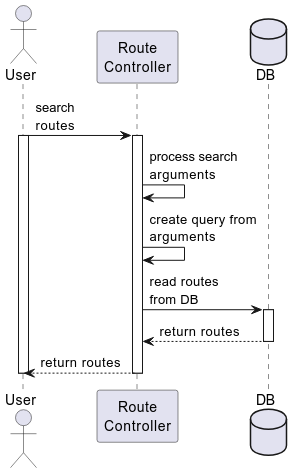
\includegraphics[width=0.3\textwidth]{model/search.png}
    \caption{Диаграмма последовательностей для поиска маршрутов}
\end{figure}

\newpage
\begin{figure}[H]
    \centering
    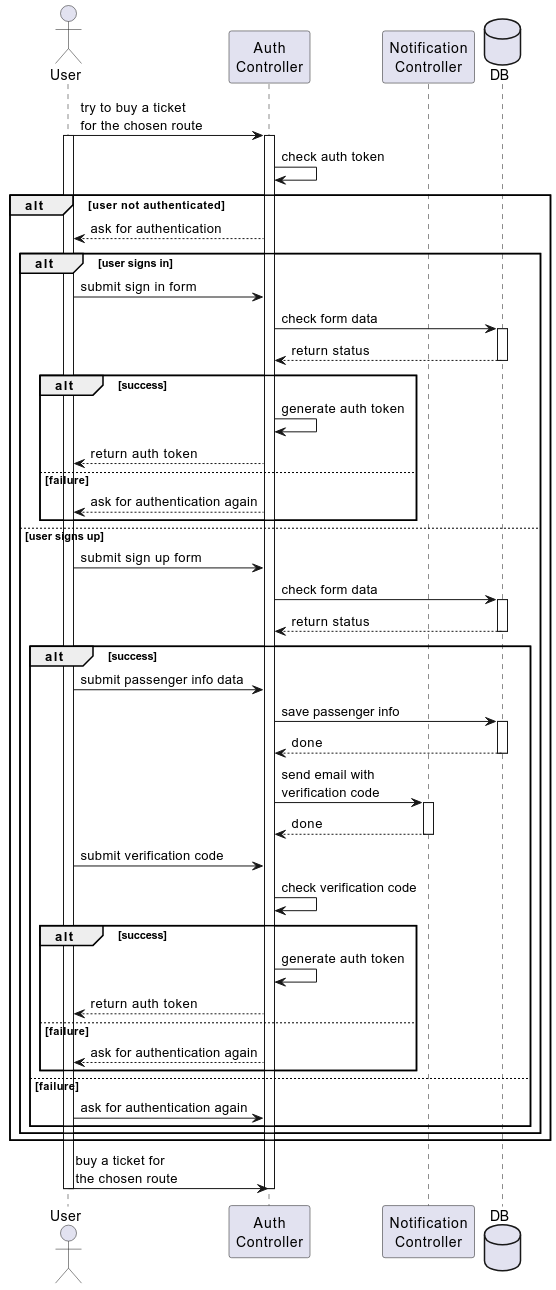
\includegraphics[width=0.5\textwidth]{model/auth.png}
    \caption{Диаграмма последовательностей для аутентификации}
\end{figure}

\newpage
\begin{figure}[H]
    \centering
    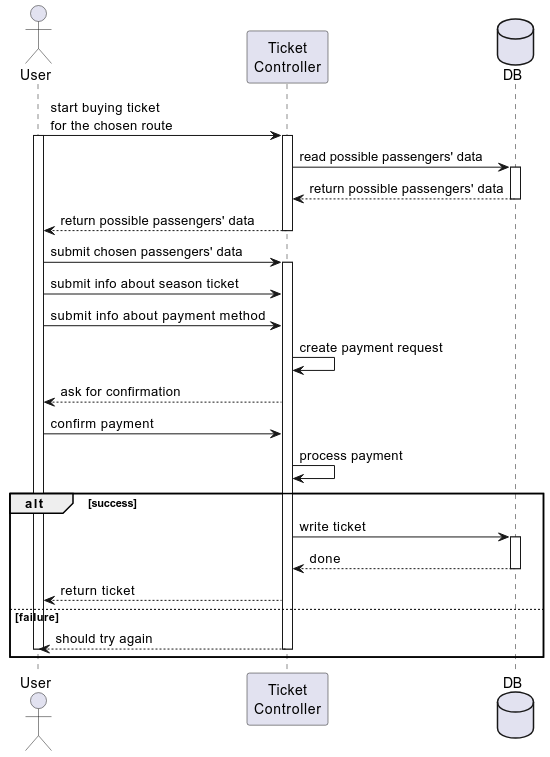
\includegraphics[width=0.5\textwidth]{model/buy.png}
    \caption{Диаграмма последовательностей для покупки билета}
\end{figure}

\newpage
\begin{figure}[H]
    \centering
    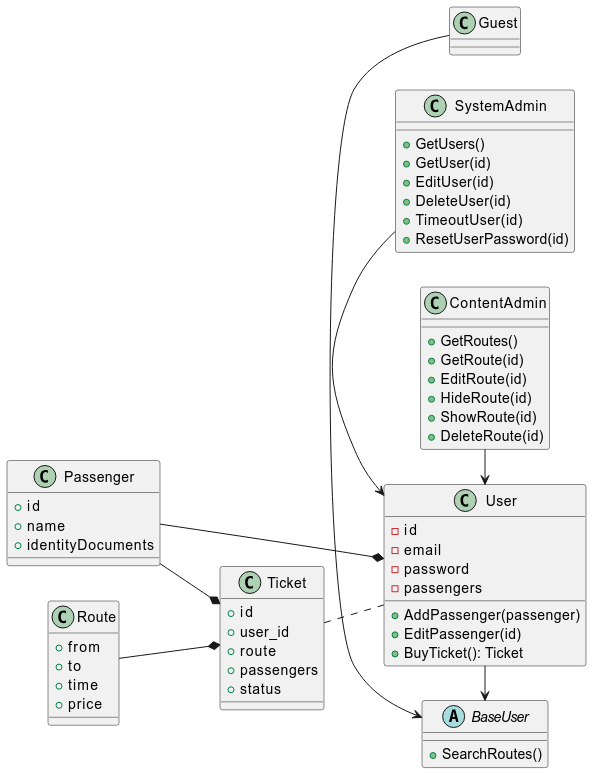
\includegraphics[width=0.7\textwidth]{model/class.png}
    \caption{Диаграмма классов}
\end{figure}


\newpage
\section{Создание объектной модели на основе методологии IDEF4}
\begin{figure}[H]
    \centering
    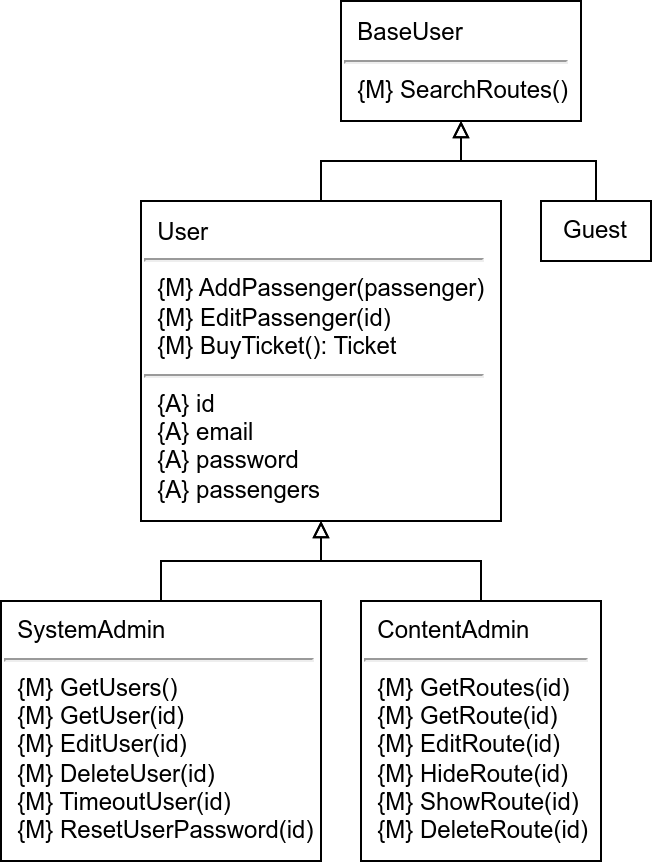
\includegraphics[width=0.5\textwidth]{model/static.png}
    \caption{Статическая модель}
\end{figure}

\newpage
\begin{figure}[H]
    \centering
    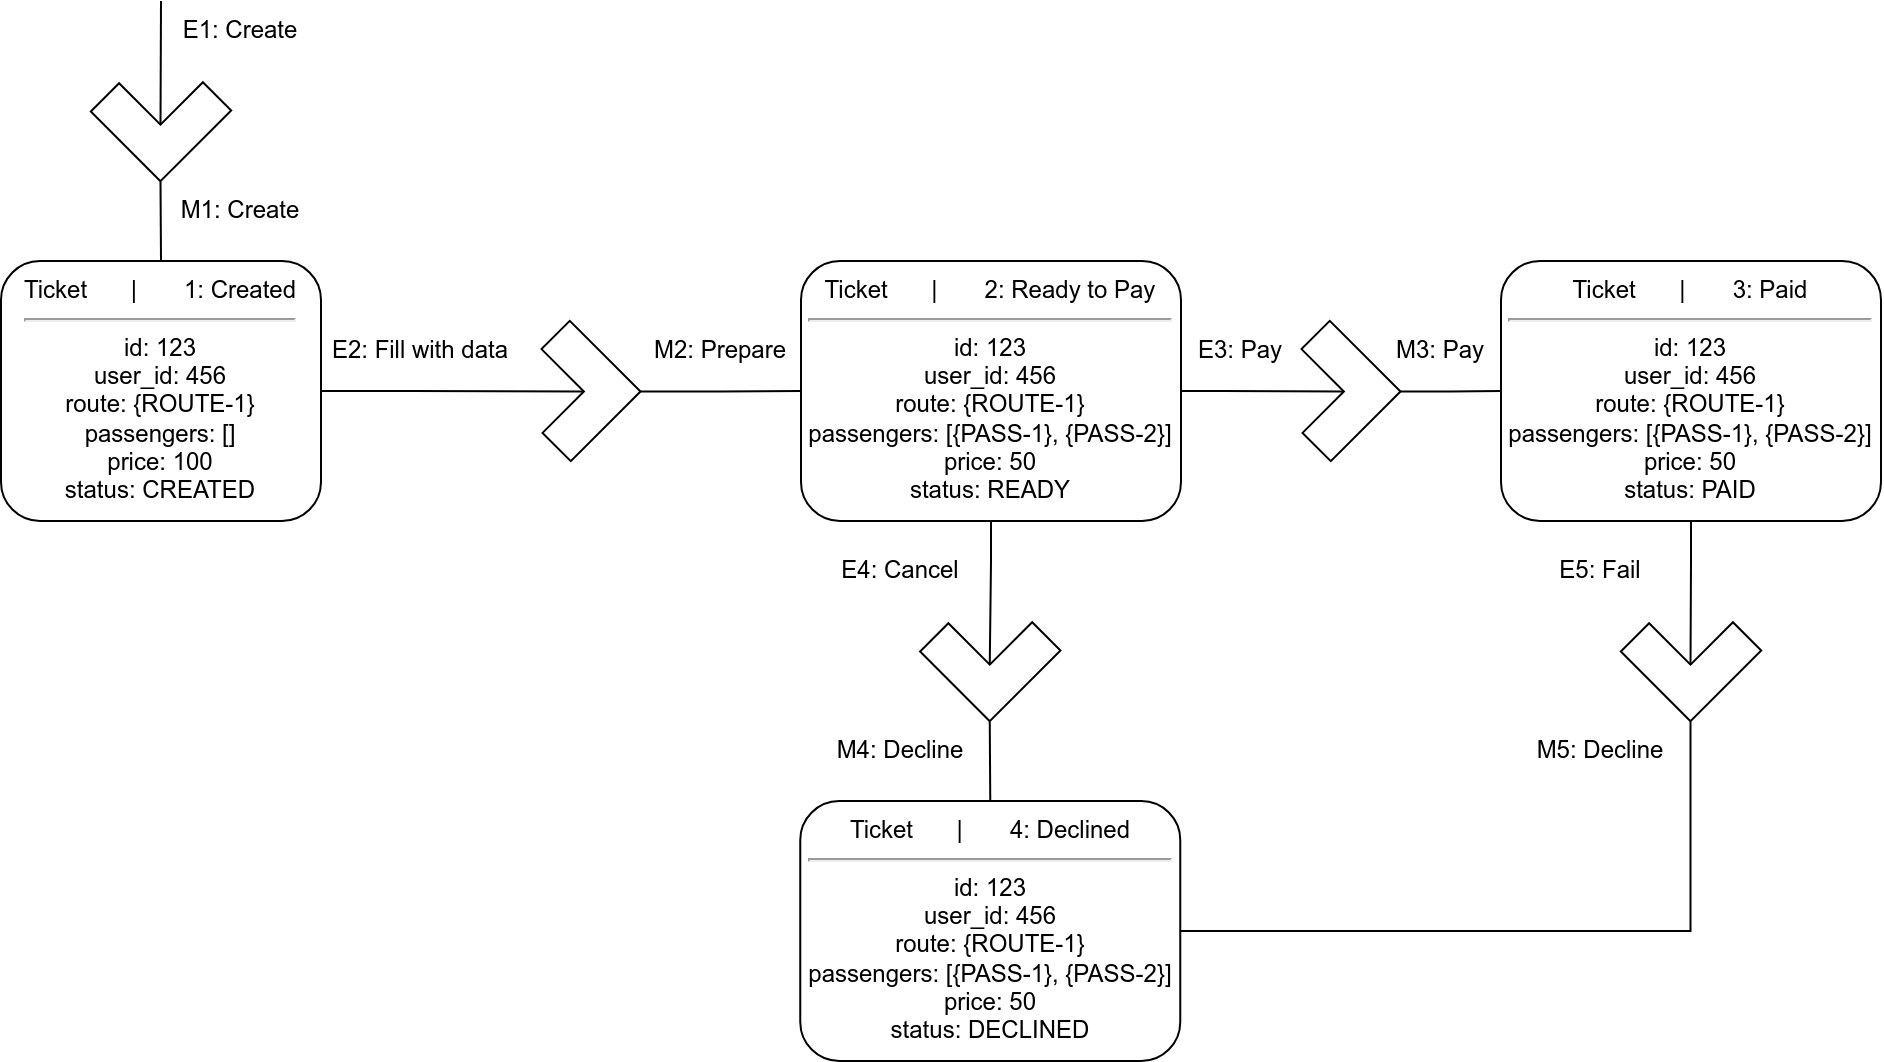
\includegraphics[width=0.9\textwidth]{model/dynamic.png}
    \caption{Динамическая модель}
\end{figure}

\newpage
\begin{figure}[H]
    \centering
    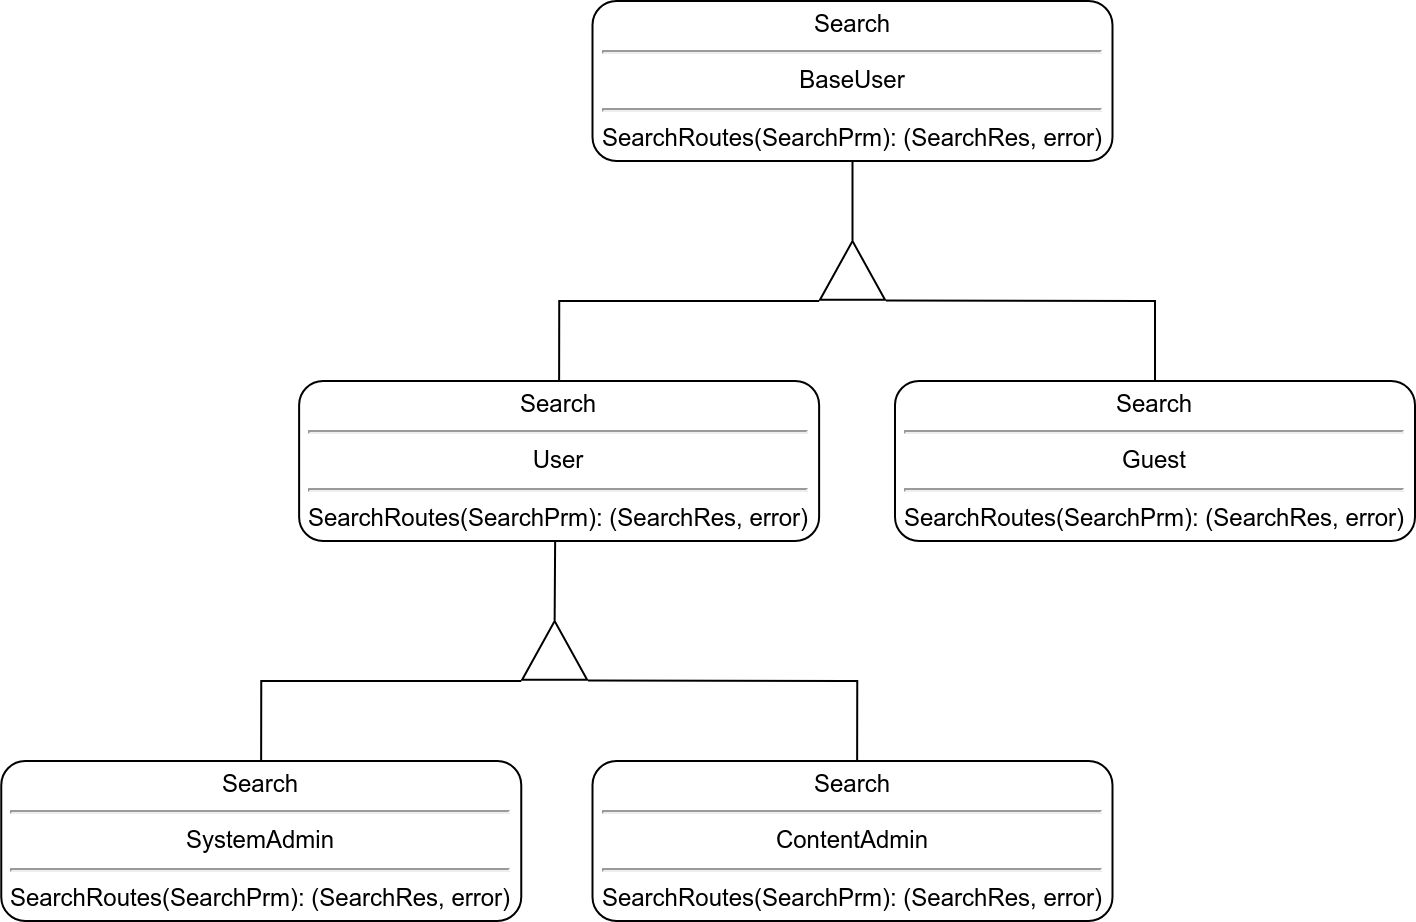
\includegraphics[width=0.9\textwidth]{model/behavior.png}
    \caption{Модель поведения}
\end{figure}


\newpage
\section*{\MakeUppercase{Заключение}}\label{sec:conclusion}
\addcontentsline{toc}{section}{Заключение}
В рамках данной работы для разработанной ранее диаграммы классы были реализованы
классы с применением шаблонов проектирования GoF (Gang of Four), что позволило
улучшить архитектуру системы, обеспечив гибкость, расширяемость и повторное использование
компонентов.

\end{document}
